\documentclass[letterpaper,12pt]{article}
\usepackage[margin=64pt]{geometry}
\usepackage{amsthm}
\usepackage{amsmath}
\usepackage{amssymb}
\usepackage{parskip}
\usepackage{graphicx}
\usepackage{enumerate}
\usepackage{hyperref}
\usepackage{listings}
\newcommand{\transpose}{^{\mbox{\tiny T}}}


\begin{document}
\thispagestyle{empty}

\hrule \vspace{0.5em}
\noindent {\bf CFRM 462: Introduction to Computational Finance and Econometrics} \hfill Homework 5 \newline \hrule

\vspace{1em}
\begin{enumerate}
\item Monte Carlo Simulation in the CER Model
\subitem{a)}
        \begin{table}[ht]
        \caption{Parameter Estimates} % title of Table
        \centering % used for centering table
        \begin{tabular}{c c c c } % centered columns (4 columns)
        \hline\hline %inserts double horizontal lines
        Asset & $\mu_{i}$ & $\sigma^2_{i}$ & $\sigma_{i}$ \\ [0.5ex] % inserts table
        %heading
        \hline % inserts single horizontal line
        VBISX & 0.00428 & 3.99e-05 & 0.00632 \\
        FBGRX & 0.00214 & 3.34e-03 & 0.05783 \\
        GOOGL & 0.00846 & 1.05e-02 & 0.10250 \\ [1ex] % [1ex] adds vertical space
        \hline %inserts single line
        \end{tabular}
        \label{table:nonlin} % is used to refer this table in the text
        \end{table}
        
        \begin{table}[ht]
        \caption{Parameter Estimates Matrix} % title of Table
        \centering % used for centering table
        \begin{tabular}{c c c c} % centered columns (4 columns)
        \hline\hline %inserts double horizontal lines
        Parameters & VBISX,FBGRX & VBISX,GOOGL & FBGRX,GOOGL \\ [0.5ex] % inserts table
        %heading
        \hline % inserts single horizontal line
        $\sigma_{ij}$  & -1.69e-05  & -1.98e-04  &  3.82e-03 \\
        $\rho_{ij}$ &  -0.0464  & -0.3065  &  0.6450  \\ [1ex] % [1ex] adds vertical space   
        \hline %inserts single line
        \end{tabular}
        \label{table:nonlin} % is used to refer this table in the text
        \end{table}
        
\subitem{b)}

        \begin{lstlisting}
                      VBISX   FBGRX   GOOGL
        muhat.vals 0.004282 0.00214 0.00846
        se.muhat   0.000815 0.00747 0.01323
        
                          VBISX    FBGRX   GOOGL
        sigma2hat.vals 3.99e-05 0.003345 0.01051
        se.sigma2hat   7.28e-06 0.000611 0.00192
        
                         VBISX   FBGRX   GOOGL
        sigmahat.vals 0.006316 0.05783 0.10250
        se.sigmahat   0.000577 0.00528 0.00936
        
                    VBISX,FBGRX VBISX,GOOGL FBGRX,GOOGL
        rhohat.vals     -0.0464      -0.306      0.6450
        se.rhohat        0.1288       0.117      0.0754
        \end{lstlisting}
        
	$\mu$ is precise for VBISX, but not for FBGRX and GOOGL. $\sigma_2$ and $\sigma$ are precise for all the assets. $\rho$ is only precise for FBGRX, GOOGL.

\subitem{c)} 
The distribution for the mean looks slightly positively skewed, but for the most part looks normally distributed. The variance looks very positively skewed and the sd looks normally distributed. \\ 
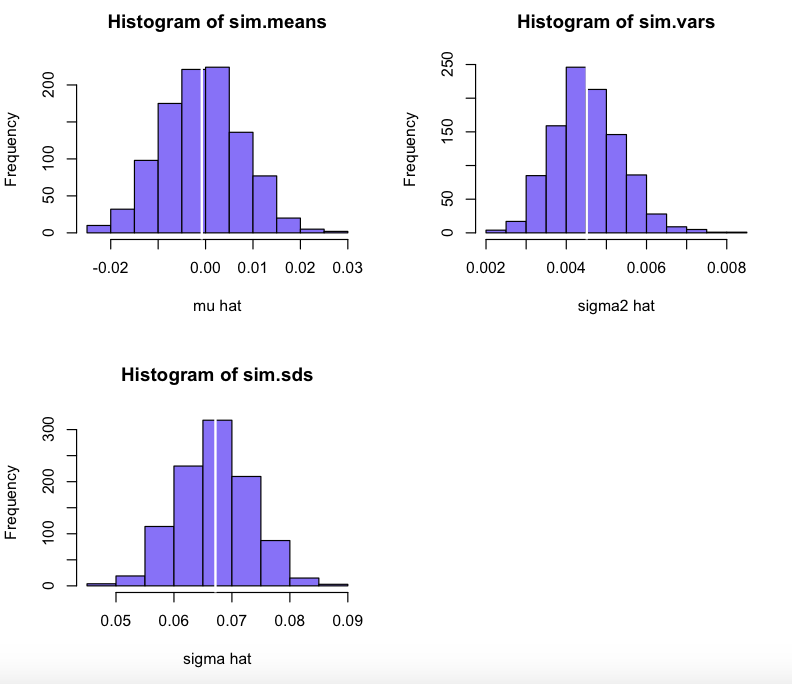
\includegraphics[scale= 0.5]{Histograms} 

The Monte Carlo simulations do a good job of estimating the parameters and all of the parameters are close to their true values. \\ 
\begin{lstlisting}
        > c(mu, mean(sim.means))
        [1] -0.000800 -0.000771
        > mean(sim.means) - mu
        [1] 2.9e-05
        > c(sd^2, mean(sim.vars))
        [1] 0.00451 0.00453
        > mean(sim.vars) - sd^2
        [1] 2.33e-05
        > c(sd, mean(sim.sds))
        [1] 0.0672 0.0670
        > mean(sim.sds) - sd
        [1] -0.000117
        > c(se.muhat["FBGRX"], sd(sim.means))
          FBGRX         
        0.00747 0.00831 
        > c(se.sigma2hat["FBGRX"], sd(sim.vars)) 
           FBGRX          
        0.000611 0.000843 
        > c(se.sigmahat["FBGRX"], sd(sim.sds))
          FBGRX         
        0.00528 0.00625
\end{lstlisting}

\item Bootstrapping

\subitem{a)}
All of the SE below are very close to the analytic solutions. 
\begin{lstlisting}
boot(data = VBISX, statistic = mean.boot, R = 999)
Bootstrap Statistics :
    original  bias    std. error
t1*  0.00428 1.6e-05    0.000807
> se.muhat["VBISX"]
   VBISX 
0.000815 

boot(data = VBISX, statistic = sd.boot, R = 999)

Bootstrap Statistics :
    original    bias    std. error
t1*  0.00632 -8.42e-05    0.000714
> se.sigmahat["VBISX"]
   VBISX 
0.000577

boot(data = VBISX, statistic = var.boot, R = 999)

Bootstrap Statistics :
    original    bias    std. error
t1* 3.99e-05 -7.31e-07    8.63e-06
> se.sigma2hat["VBISX"]
   VBISX 
7.28e-06

boot(data = ret.mat[, c("VBISX", "FBGRX")], statistic = rho.boot, 
    R = 999)


Bootstrap Statistics :
    original  bias    std. error
t1*  -0.0464  0.0036        0.16
> se.rhohat[1]
VBISX,FBGRX 
      0.129 
\end{lstlisting}
\subitem{b)} The mean looks relatively normally distributed, except it is slightly negatively skewed and the qq plot has non-normal behavior in the lower quantiles. The sd does not look symmetric about the mean and exhibits non-normal behavior in the lower quantiles of the qq plot. The var looks almost bimodal and exhibits non-normal behavior in the lower quantiles of the qq plot. Rho looks the most normal because it is almost symmetric and the qq plot is very linear. \\ 
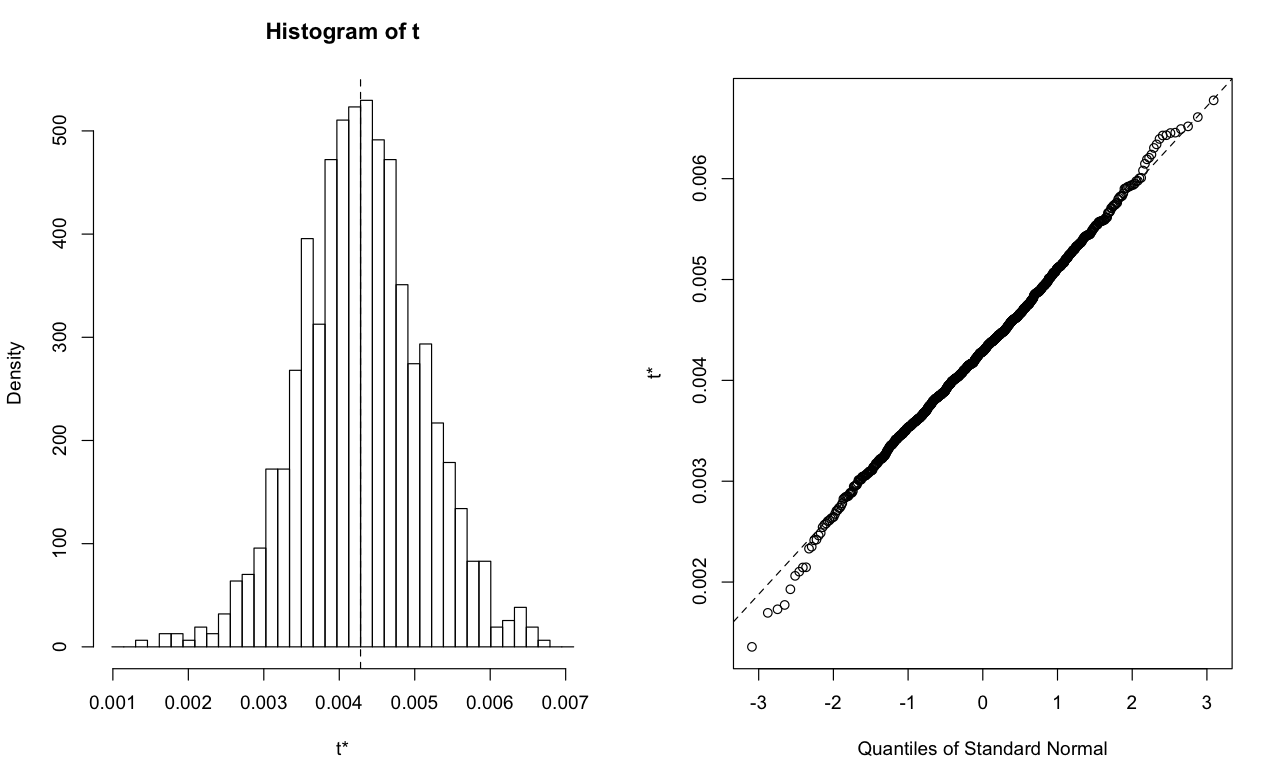
\includegraphics[scale = 0.3]{mean} \\ 
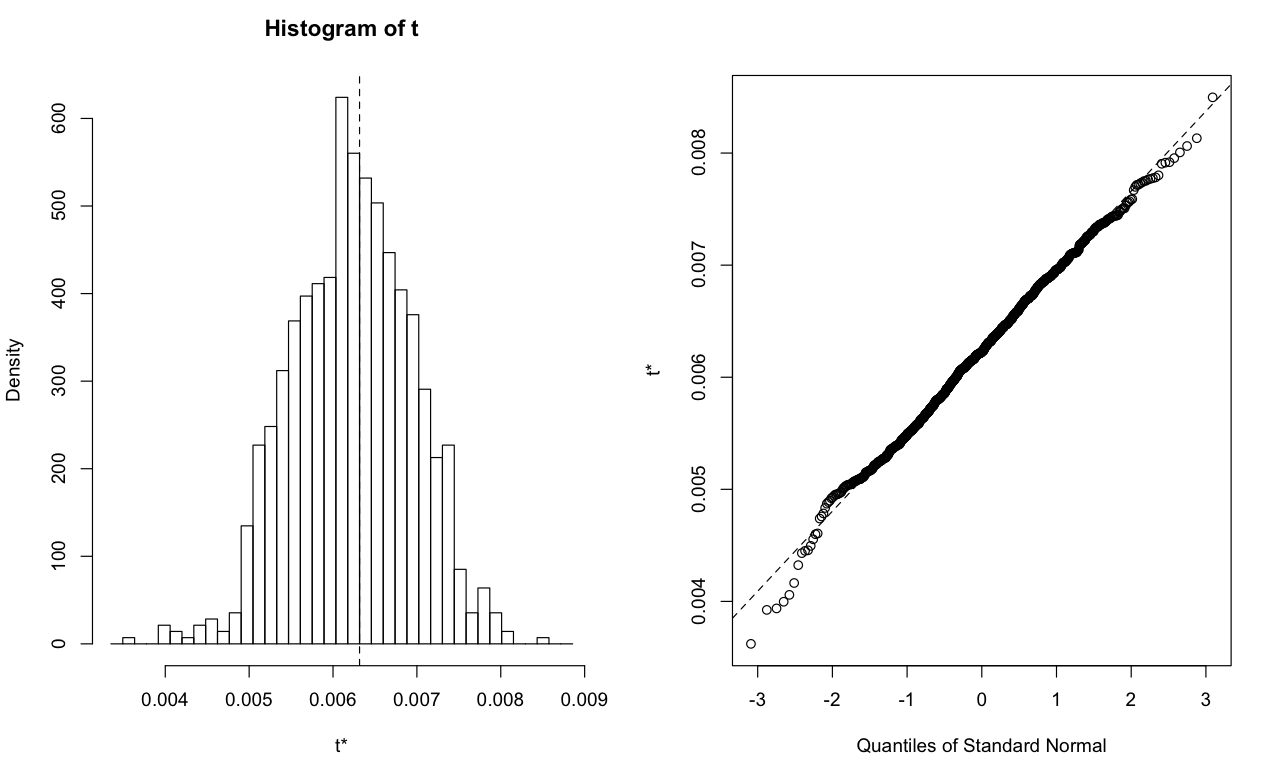
\includegraphics[scale = 0.3]{sd} \\
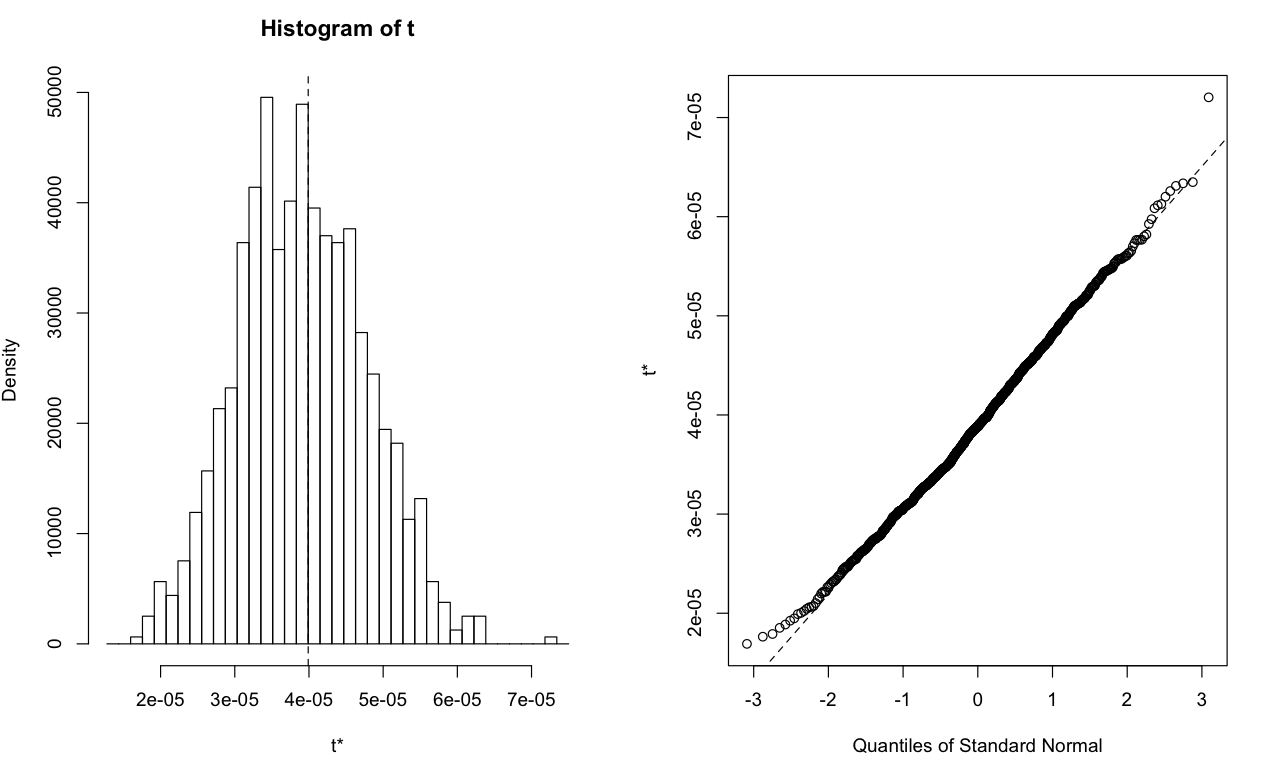
\includegraphics[scale = 0.3]{var} \\
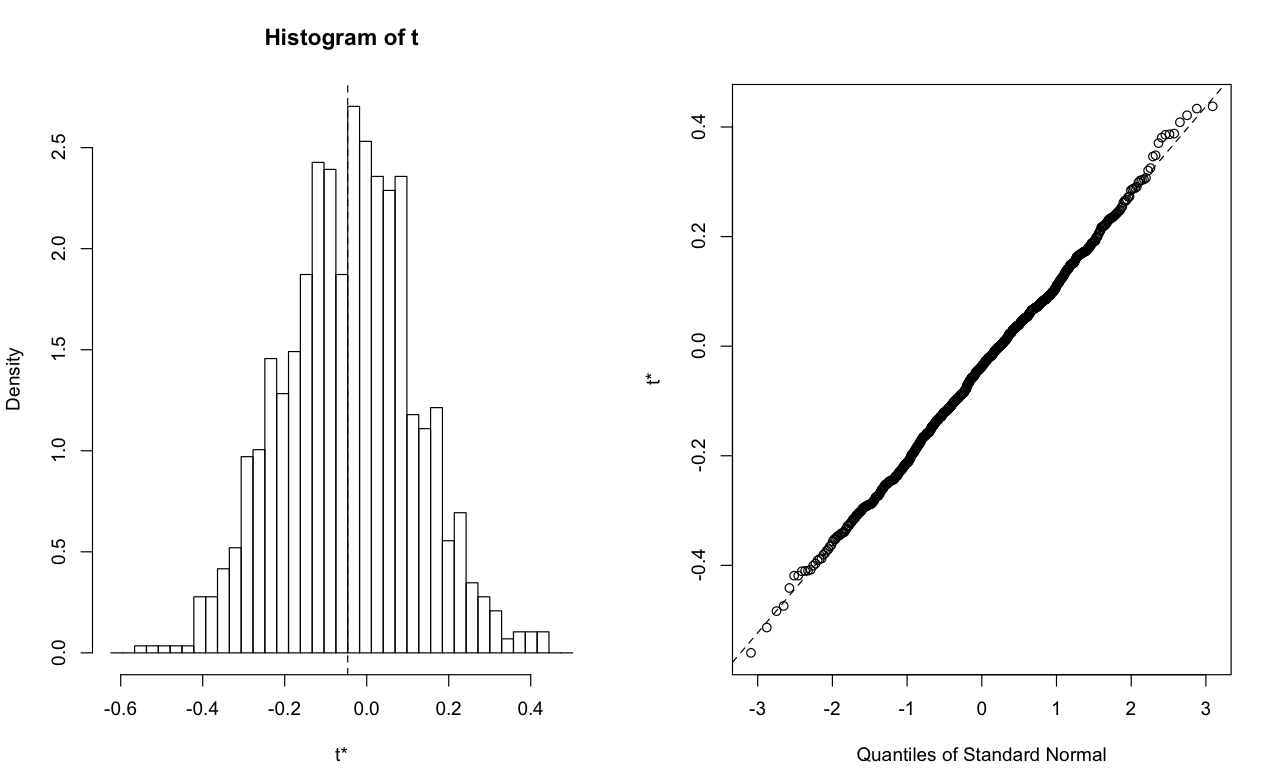
\includegraphics[scale = 0.3]{rho} \\

\subitem{c)} The bootstrap estimate suggests only a small loss and error of 131, also the confidence interval is fairly small
        \begin{lstlisting}
        boot(data = VBISX, statistic = ValueAtRisk.boot, R = 999)
        
        
        Bootstrap Statistics :
            original  bias    std. error
        t1*     -609    9.76         131
        
        boot.ci(boot.out = VBISX.VaR.boot, conf = 0.95, type = c("norm", 
            "perc"))
        
        Intervals : 
        Level      Normal             Percentile     
        95%   (-888, -354)   (-875, -335) 
        \end{lstlisting}
        
\item Class Project
\subitem{a)} The parameter estimates for mu are much less accurate than sigma, which is clear from the wide confidence intervals that include both negative and positive numbers as well as the magnitude of the SE compared to mu. Sigma and sigma2 are relatively accurate, the SE is very small. However, sigma2 has a much larger confidence interval, which suggests the se is not very accurate.

\begin{lstlisting}
#Compute se for mean
nobs = nrow(ret.mat)
se.muhat = sd.vals/sqrt(nobs)

# compute approx 95% confidence intervals
mu.lower = muhat.vals - 2*se.muhat
mu.upper = muhat.vals + 2*se.muhat

#Sigma SE
se.sigma = sd.vals/sqrt(2*nobs)

sigma.lower = sd.vals - 2 * se.sigma
sigma.upper = sd.vals + 2 * se.sigma

#Var SE
se.sigma2 = sd.vals/sqrt(nobs/2)

sigma2.lower = var.vals - 2 * se.sigma2
sigma2.upper = var.vals + 2 * se.sigma2

#Cov SE

#Cor SE
se.rho = (1-rhohat.vals)^2/sqrt(nobs)

rho.lower = rhohat.vals - 2 * se.rho
rho.upper = rhohat.vals + 2 * se.rho

#Combine the SE
rbind(se.muhat,se.sigma,se.sigma2,se.rho)

vfinx   presx   hlemx   vbllx    fshbx   vpacx
se.muhat  0.00425 0.00611 0.00619 0.00306 0.000290 0.00501
se.sigma  0.00301 0.00432 0.00438 0.00216 0.000205 0.00354
se.sigma2 0.00601 0.00864 0.00875 0.00432 0.000410 0.00708

rbind(mu.lower,mu.upper,sigma.lower,sigma.upper)

                vfinx    presx    hlemx     vbllx     fshbx    vpacx
mu.lower      0.00303 -0.00457 -0.00935  0.000462  0.000726 -0.00538
mu.upper      0.02003  0.01987  0.01541  0.012689  0.001885  0.01465
sigma.lower   0.03005  0.04320  0.04377  0.021616  0.002050  0.03540
sigma.upper   0.04207  0.06047  0.06128  0.030262  0.002870  0.04955
sigma2.lower -0.01072 -0.01459 -0.01475 -0.007973 -0.000814 -0.01235
sigma2.upper  0.01332  0.01997  0.02027  0.009319  0.000826  0.01596

\end{lstlisting}
\end{enumerate}
\vfill \hrule \vspace{2mm} \centerline {\tt \tiny http://computational-finance.uw.edu}
\end{document}